\chapter{多铁材料与多铁性}


\section{多铁材料的研究背景}

铁性质,最早来源于对铁磁性的研究,后来有些电介质被发现存在与铁磁性的显著特征相似的性质,于是这种类似于铁磁性的性质被命名为铁电性,拥有这些性质的材料也被称为铁电材料,尽管有些材料与铁元素没有任何关系。多铁材料是指在一个单一的相之中存在两个及以上的铁性质,例如铁磁、铁电铁、弹性、铁环性。\cite{eerenstein2006multiferroic} 目前通常指代将磁性行为与铁电相结合的电磁材料。\cite{spaldin2019advances} 多铁材料内部同时存在的铁磁性与铁电性或许可以将电场与磁场进行耦合是研究多铁材料的一个重要原因。自从麦克斯韦方程组建立以来,人们早已认识到电磁并不是孤立存在的两种事物,联系是客观的普遍存在的,而是有联系的并可以进行相互转化。安培环路定理、位移电流、法拉第电磁感应定律表明,变化的电场产生变化的磁场、变化的磁场会激发变化的电场。\cite{刘俊明2019多铁性} 然而,在铁电和铁磁两个领域,电与磁的界限依然十分明显,几乎没有同时具有强铁电性与强铁磁性的材料。

\begin{figure}[h]
    \centering
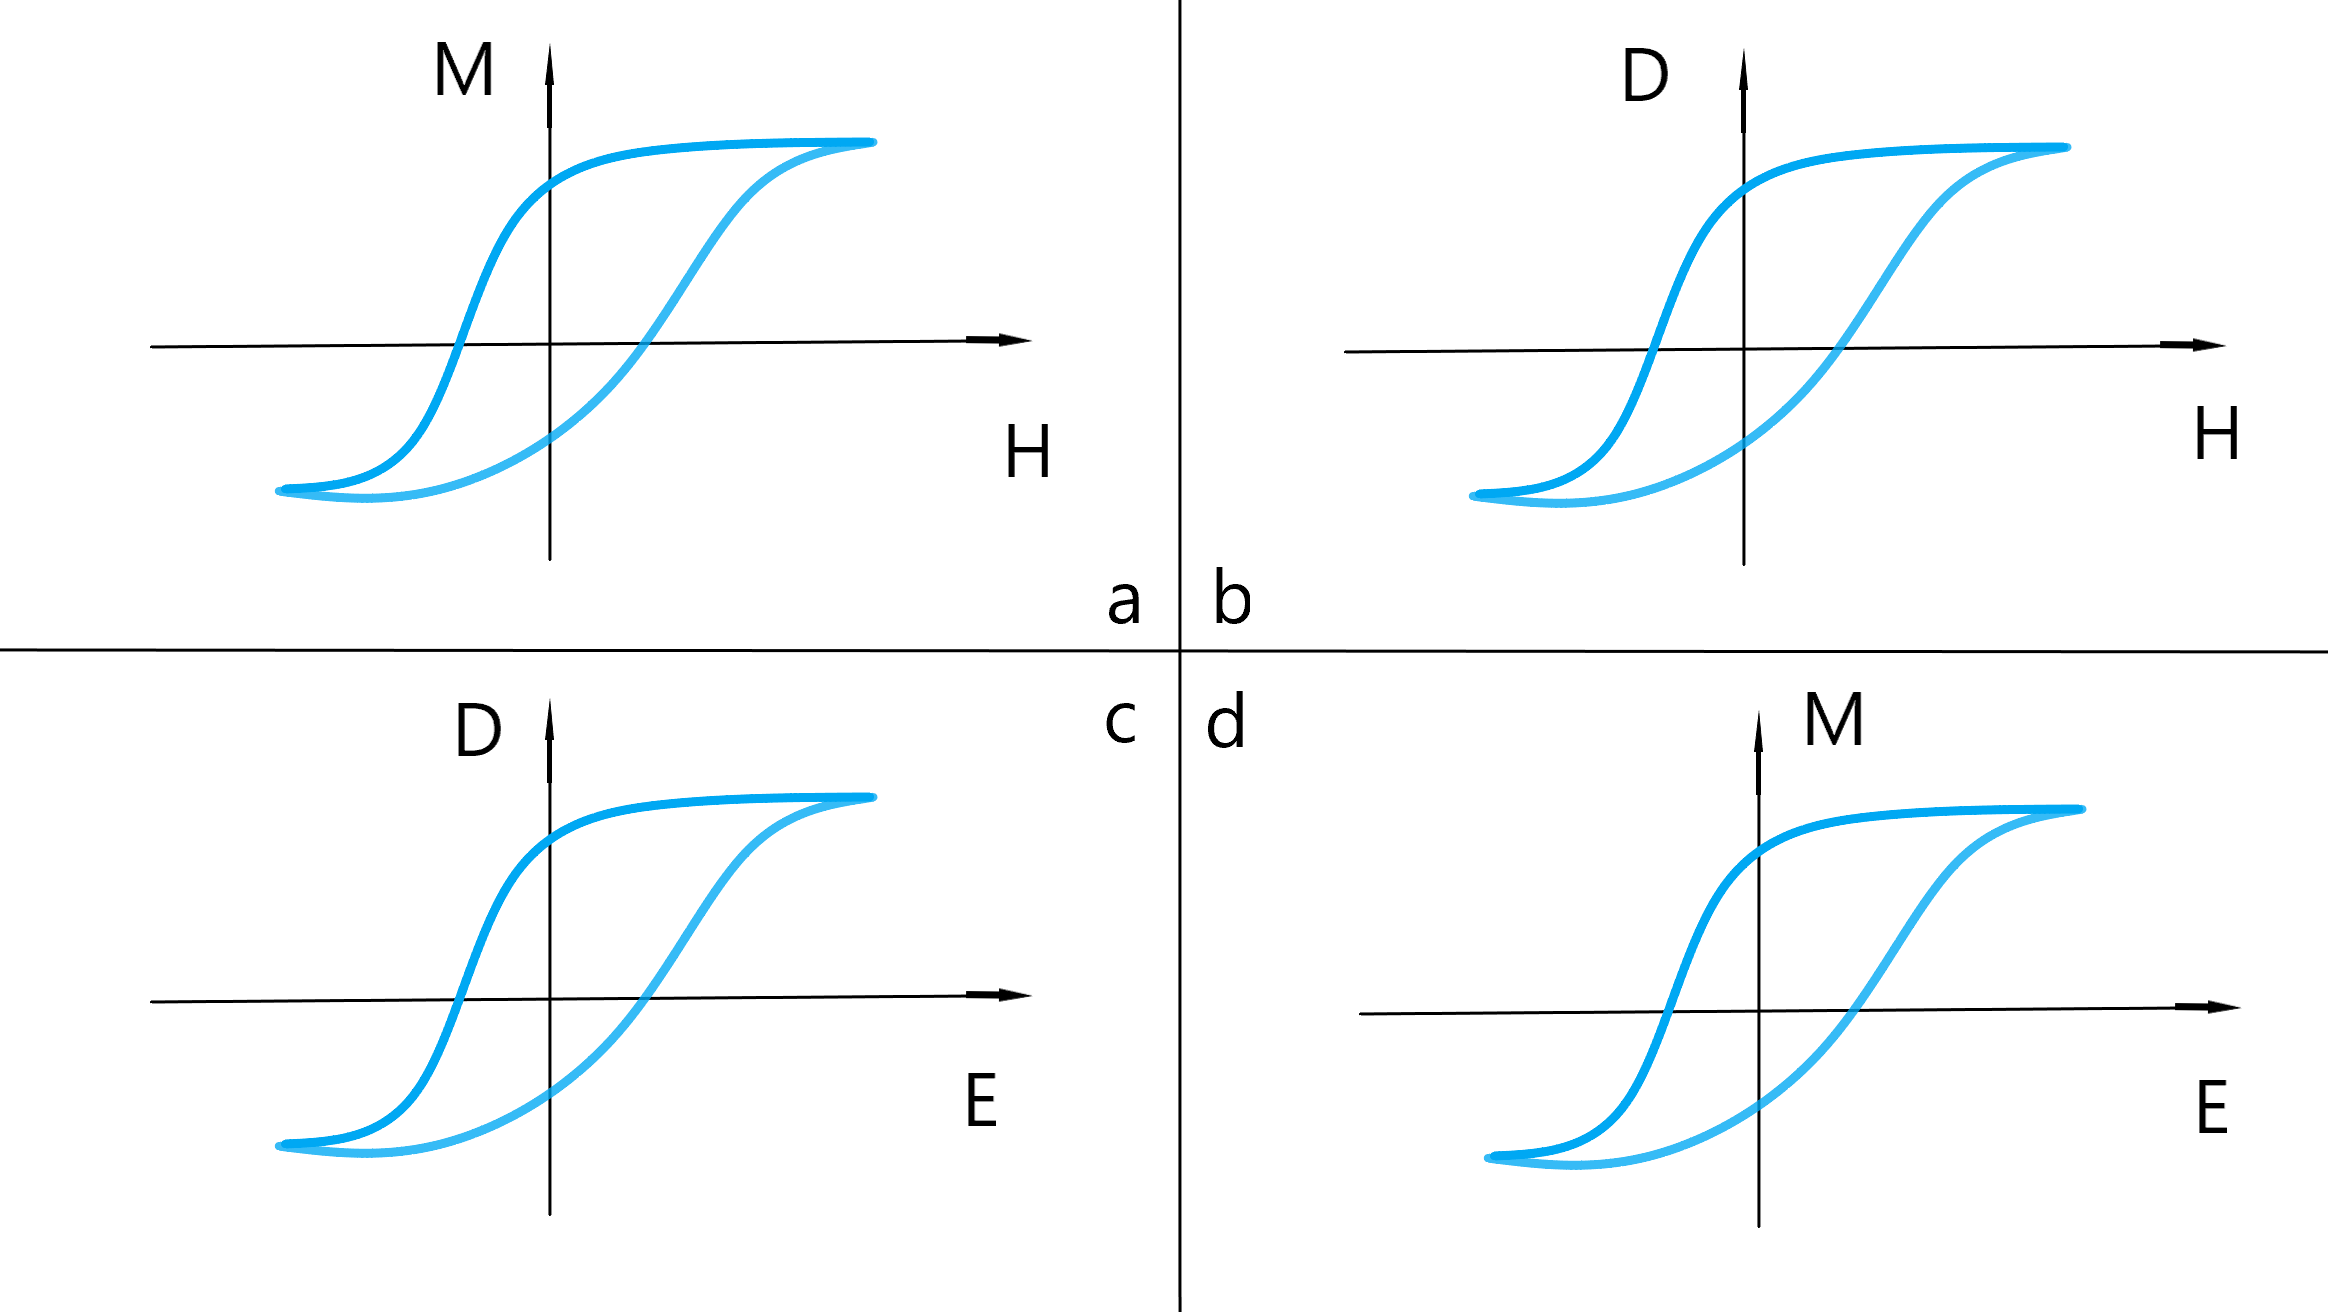
\includegraphics[width=0.8\textwidth]{./pic/003.png}
\caption{铁磁性、铁电性、多铁性示意图  (a)(c)是传统的铁磁性与铁电性,外加磁场可以使铁磁性物质出现磁矩,外加电场会使铁电性物质出现电极化。在外场撤出之后,受外场影响所产生的磁矩与电极化并不会消失。(b)(d)是多铁性材料铁电与铁磁性质的耦合,通过外加电场可以使诱导出宏观磁矩,外加磁场可以产生出电极化。}

\label{dog003}
\end{figure}

\section{多铁材料的基本原理}

多铁材料,一般来说是指同时具有铁电性与铁磁性的材料,结构决定性质,两种性质同时存在必然要求具有能够支撑适应铁电与铁磁的的特殊的微观结构。

\begin{figure}[h]
    \centering
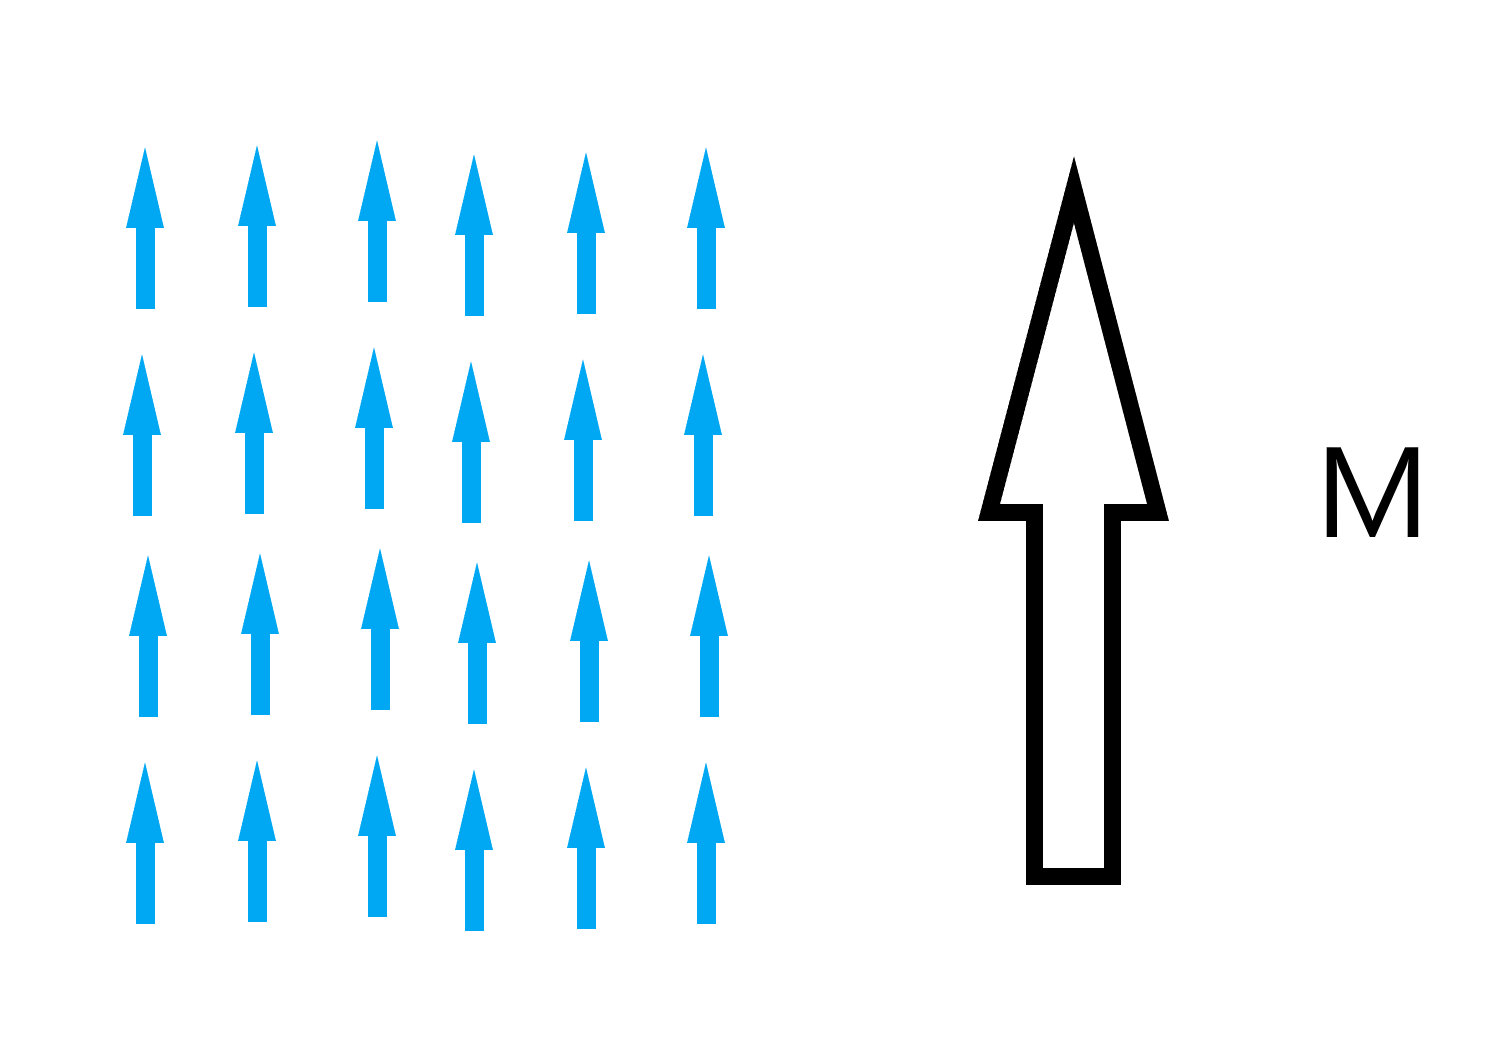
\includegraphics[width=0.8\textwidth]{./pic/001.png}
\caption{铁磁性物质磁化后的微观图像:微观磁矩平行排列,在宏观尺度上表现出磁矩。}
\label{dog001}
\end{figure}

\subsection{铁磁性的来源}

从经典的以麦克斯韦方程组为基础的电磁理论认为,恒定的电流产生恒定的磁场,变化的电流产生变化的磁场。在固体物理领域一般认为,固体的磁性来自电子的轨道运动,电子自身带有自旋、磁矩。固体在宏观上出现磁性微观原因是固体内部的磁有序。从对称性上面看,铁磁性的出现是时间反演对称性的破缺,磁矩产生自电荷的运动,在时间反演下,磁矩会改变方向。经典的看法是,铁磁性材料中的磁矩来源于原子中的未配对电子,通常在d轨道或f轨道电子半满的原子,会产生强的铁磁性。\cite{fiebig2016the} 

\begin{figure}[h]
    \centering
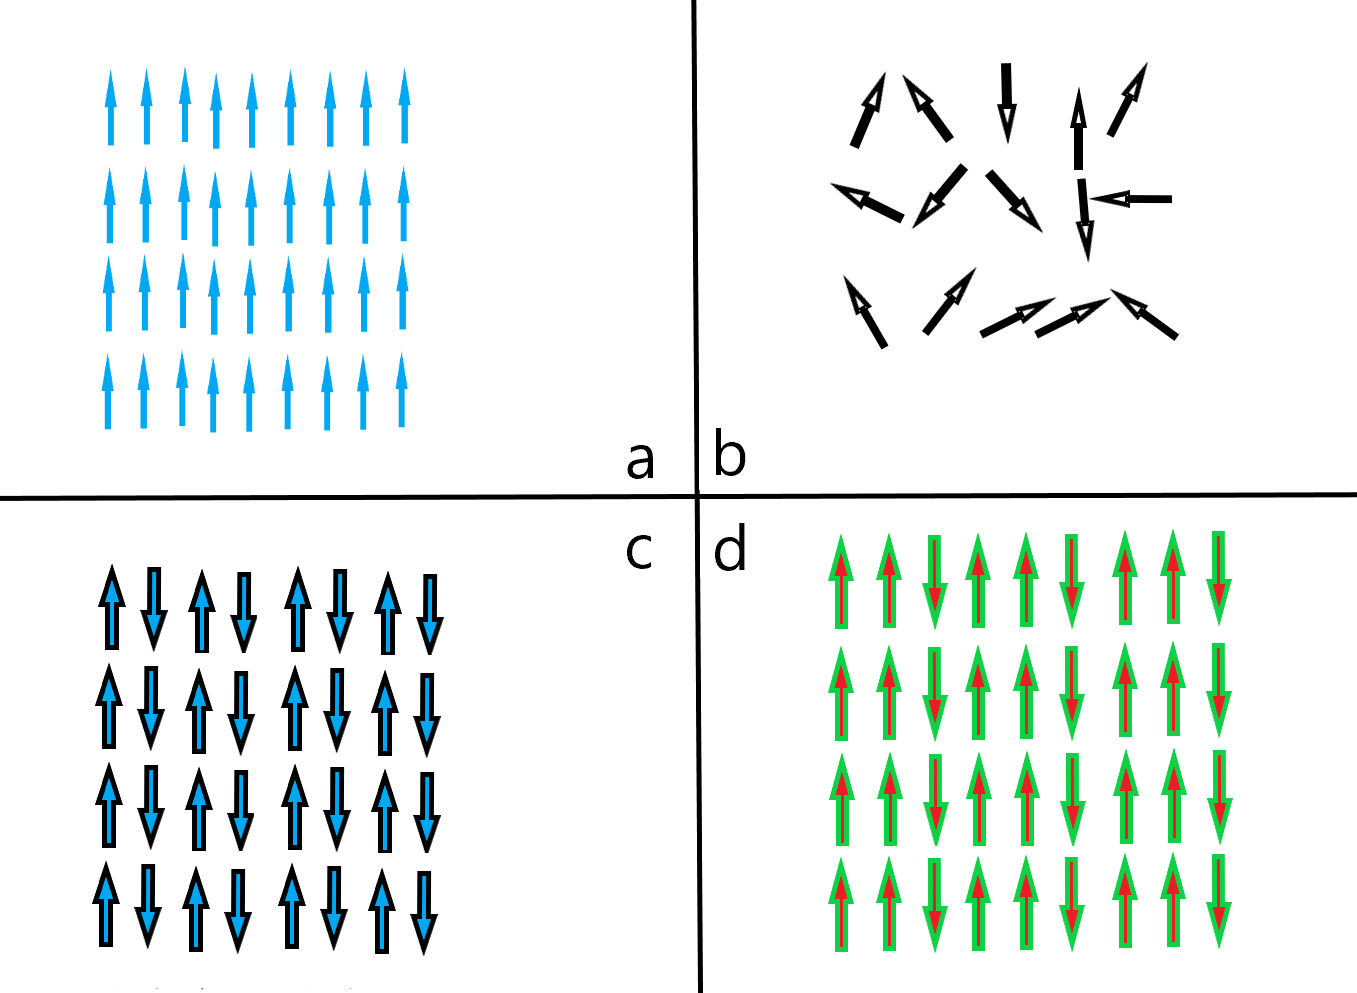
\includegraphics[width=0.8\textwidth]{./pic/002.png}
\caption{铁磁性、反铁磁性、亚铁磁性和顺磁性的微观磁矩图像  (a)是铁磁性物质的微观图像,各个微观磁矩有序排列,微观小磁矩相互叠加,在宏观上表现出宏观磁矩。(b)是具有顺磁性的物质,在无外加磁场的影响下,微观磁矩杂乱无章,随机排列,各个方向磁矩相互抵消,在宏观上不表现出磁矩。(c)是反铁磁性的微观图像,各个微观磁矩有序排列,但方向相反,各处微观磁矩相互抵消,在宏观上不表现磁矩。(d)是亚铁磁性的微观图像,微观磁矩也是规则排列,与反铁磁性不同的是,微观磁矩并没有被完全抵消,在宏观尺度仍然存在磁矩。}

\label{dog002}
\end{figure}

基于元素周期表与核外电子排布规律,传统的铁磁性材料主要来自于过渡金属元素(d电子半充满)与稀土元素(f电子半充满)。\cite{hill2000why}

\subsection{磁有序}

铁磁性的来源与磁有序密切相关,而物质的磁性与微观粒子的内部构造密切相关。磁有序,在宏观上可以产生主要包括铁磁性、反铁磁性、亚铁磁性等材料性质,磁有序的产生与自旋旋转对称性或者时间反演对称的破缺有关。引起磁性的微观粒子的自旋完全是量子力学导出的结果,通过一般经典的理论解释会十分困难,但是,在一定的近似条件或者特定的研究对象的情况下,可以将其视作宏观世界之中的矢量来处理。不同的近似会导出不同的物理模型,常见的描述微观磁现象的模型主要有XY模型、海森堡模型、Ising模型等。\cite{dong2019magnetoelectricity}

\begin{figure}[h]
    \centering
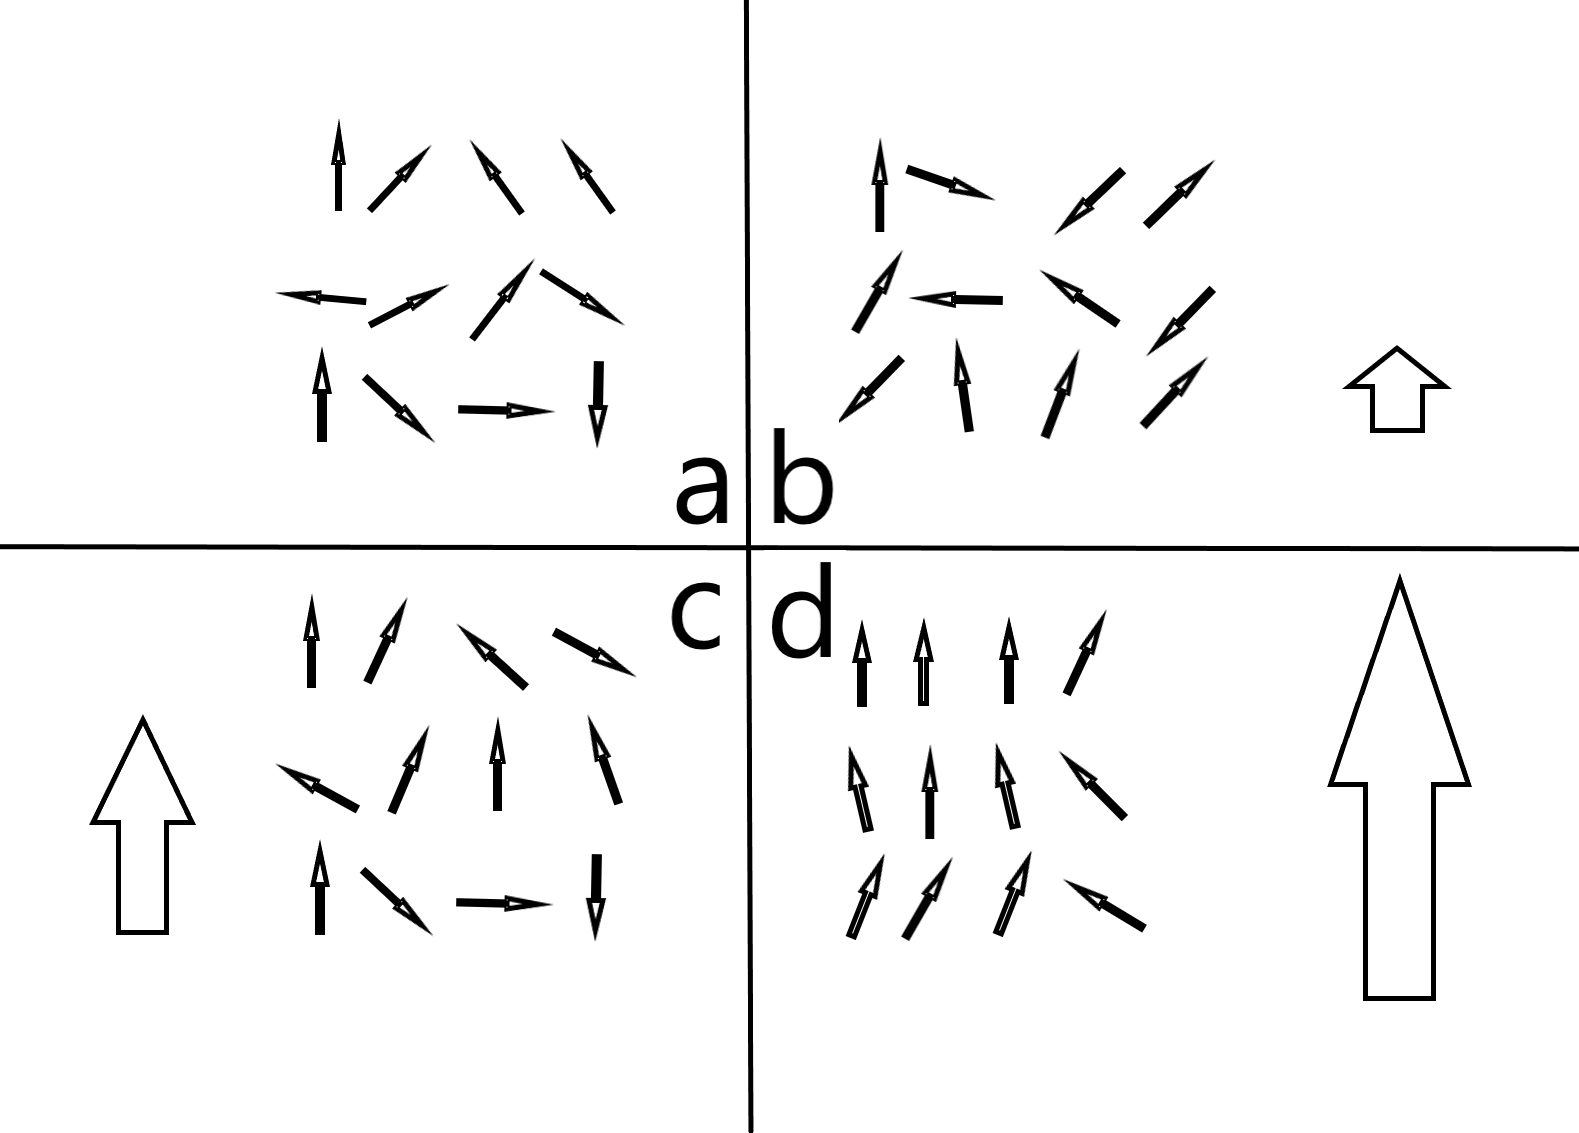
\includegraphics[width=0.8\textwidth]{./pic/005.png}
\caption{顺磁性物质微观磁矩随外场变化\ 图片从(a)到(d)随着外磁场的增加,本来混乱无序排列的微观磁矩会在外加磁场的影响下顺着外加磁场的方向排列,一般来说,外加磁场越强,磁化强度越大。与铁磁性不同的是,当外加磁场去除之后,磁化强度也会随之消失。}

\label{dog005}
\end{figure}

一般材料是由微观层面的原子组成的,原子又是由原子核与核外电子组成的。原子核的磁矩,电子自旋运动的磁矩,电子轨道运动的磁矩三种磁矩构成了原子尺度上的微观磁矩。由于质子、中子等原子核之中的重子比电子质量大三个数量级,原子核的磁矩比电子磁矩小三个数量级,在研究系统自旋磁矩的问题时通常忽略原子核的影响。\cite{王克锋2008单相多铁性材料}在过渡金属元素组成的磁性材料之中,对磁性材料的物理性质起决定性作用的是电子的自旋磁矩。金属材料电子自旋运动的行为可以根据磁化率与的大小与符号划分。
$$\chi =\mathbf{M} /\mathbf{H} $$ 
其中,$\chi$ 为磁化率,$\mathsf{M}$ 是单位体积内部所有磁矩的矢量和,H是外磁场的强度。磁有序行为可以分为五大类行:铁磁性、反铁磁性、亚铁磁性、顺磁性、抗磁性。前三种性质体现出大量磁矩合作的性质,后两种只是磁矩性质的集合。

\begin{figure}[h]
    \centering
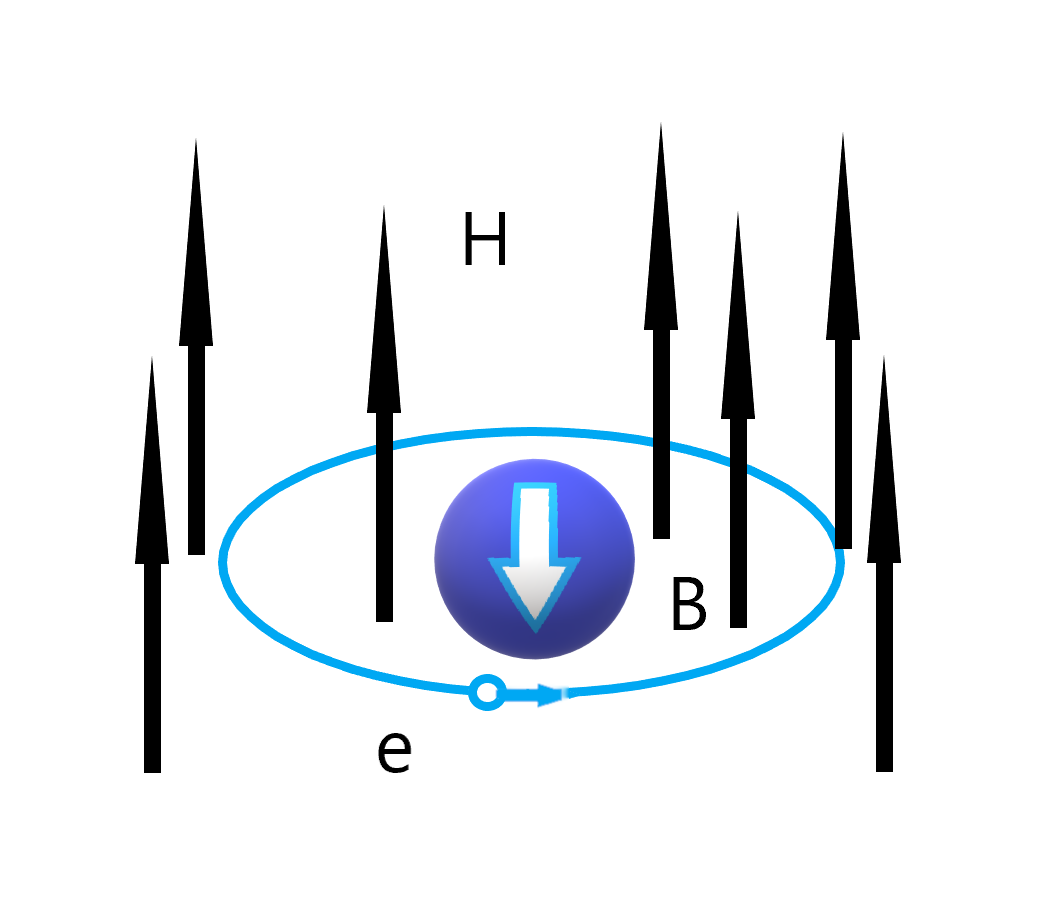
\includegraphics[width=0.8\textwidth]{./pic/004-2.png}
\caption{抗磁性 \ 物质普遍存在的抗磁性是由物质本身微观原子结构决定的。绕原子核运动的电子可以看作一个电流元,在外加磁场的作用下,绕核运动的电子会受到额外的洛伦兹力,这个洛伦兹力会使电子的绕核运动发生改变,依据楞次定律,电子运动改变的结果会削弱外加磁场的影响。}

\label{dog004}
\end{figure}

\paragraph{抗磁性}

实际上,所有的物质(由原子核与核外电子组成的)全部具有或多或少的抗磁性。抗磁性物质具有负的磁化率,一般比较微弱,同时常常被更大的顺磁性的正磁化率所掩盖。抗磁性的微观机理通常很容易解释。根据麦克斯韦方程组以及楞次定律,看作环状电流的电子绕核运动所产生的磁矩在外磁场加入后会因环状电流受外加磁场的影响而变化产生一个抵抗磁通量变化感应磁矩。根据电磁学的一般规律,这种变化是与外磁场方向相反的,普遍存在的抗磁性是经典电磁学“来拒去留”的生动体现,因此其磁化率是负的,而且与温度无关。




\paragraph{顺磁性}
很多固体,如Al、Pd等,具有一定的顺磁性。在顺磁性固体内部的磁矩,分子的无规则热运动会使磁矩无规则取向。外磁场的诱导会使得沿着磁场方向的磁矩数目会有所增加,逆着磁场方向的磁矩数目会有所减少。沿着特定方向磁矩数目的变化会导致产生一个磁化强度M,原来受到热运动影响完全等价的各个空间方向会出现一个特殊取向,即外加磁场的方向,磁矩旋转对称性会被破坏。顺磁性磁化强度是负的,而且与外磁场是线性关系,磁化强度也随外磁场撤离而消失。



\paragraph{铁磁性}
铁、钴、镍是常见的铁磁性材料。铁磁性材料通常有一个转变温度$T_{c}$,低于这个温度的情况下具有铁磁性,高于这个温度的情况下具有顺磁性。这说明在$T_{c}$以下,自旋有自发平行的取向,当温度提高之后自旋取向无规律,在$T_{c}$以上铁磁性物质的磁性行为与顺磁性物质类似,磁化率与温度关系满足居里定律。

\paragraph{反铁磁性}
常见的反铁磁性材料有铬和锰,与铁磁性物质一样反铁磁性也有一个转变温度,在转变温度以上时具有顺磁性性质,在转变温度$T_{N}$以下时,一半自旋与另一半自旋是反平行的,总磁化强度为0。

\paragraph{亚铁磁性}
铁氧体如$Fe_{3}O_{4}$是常见的亚铁磁体,与反铁磁性物质相似,在$T_{c}$以上微观磁矩无规则排列,在$T_{c}$以下,微观自旋按照反平行排列。不同的是,反平行排列的微观磁矩大小不相等,因此在宏观上是存在磁矩的。亚铁磁性物质另一个特点是在转变温度以上很大温度范围内并不遵守磁化强度与温度相关的居里定律。

这几种磁有序性质之中,最有趣最重要、应用最广的是铁磁性,尤其是其在外加磁场撤除之后的磁滞回线。这几种磁有序虽然在性质特点与磁性行为上各有不同,但在本质上是有共同点的,是同一种物理规则支配下的不同表现形式,磁有序结构归根究底是晶格上的离子磁矩以及离域电子磁矩的直接或间接的相互作用。

\begin{figure}[h]
    \centering
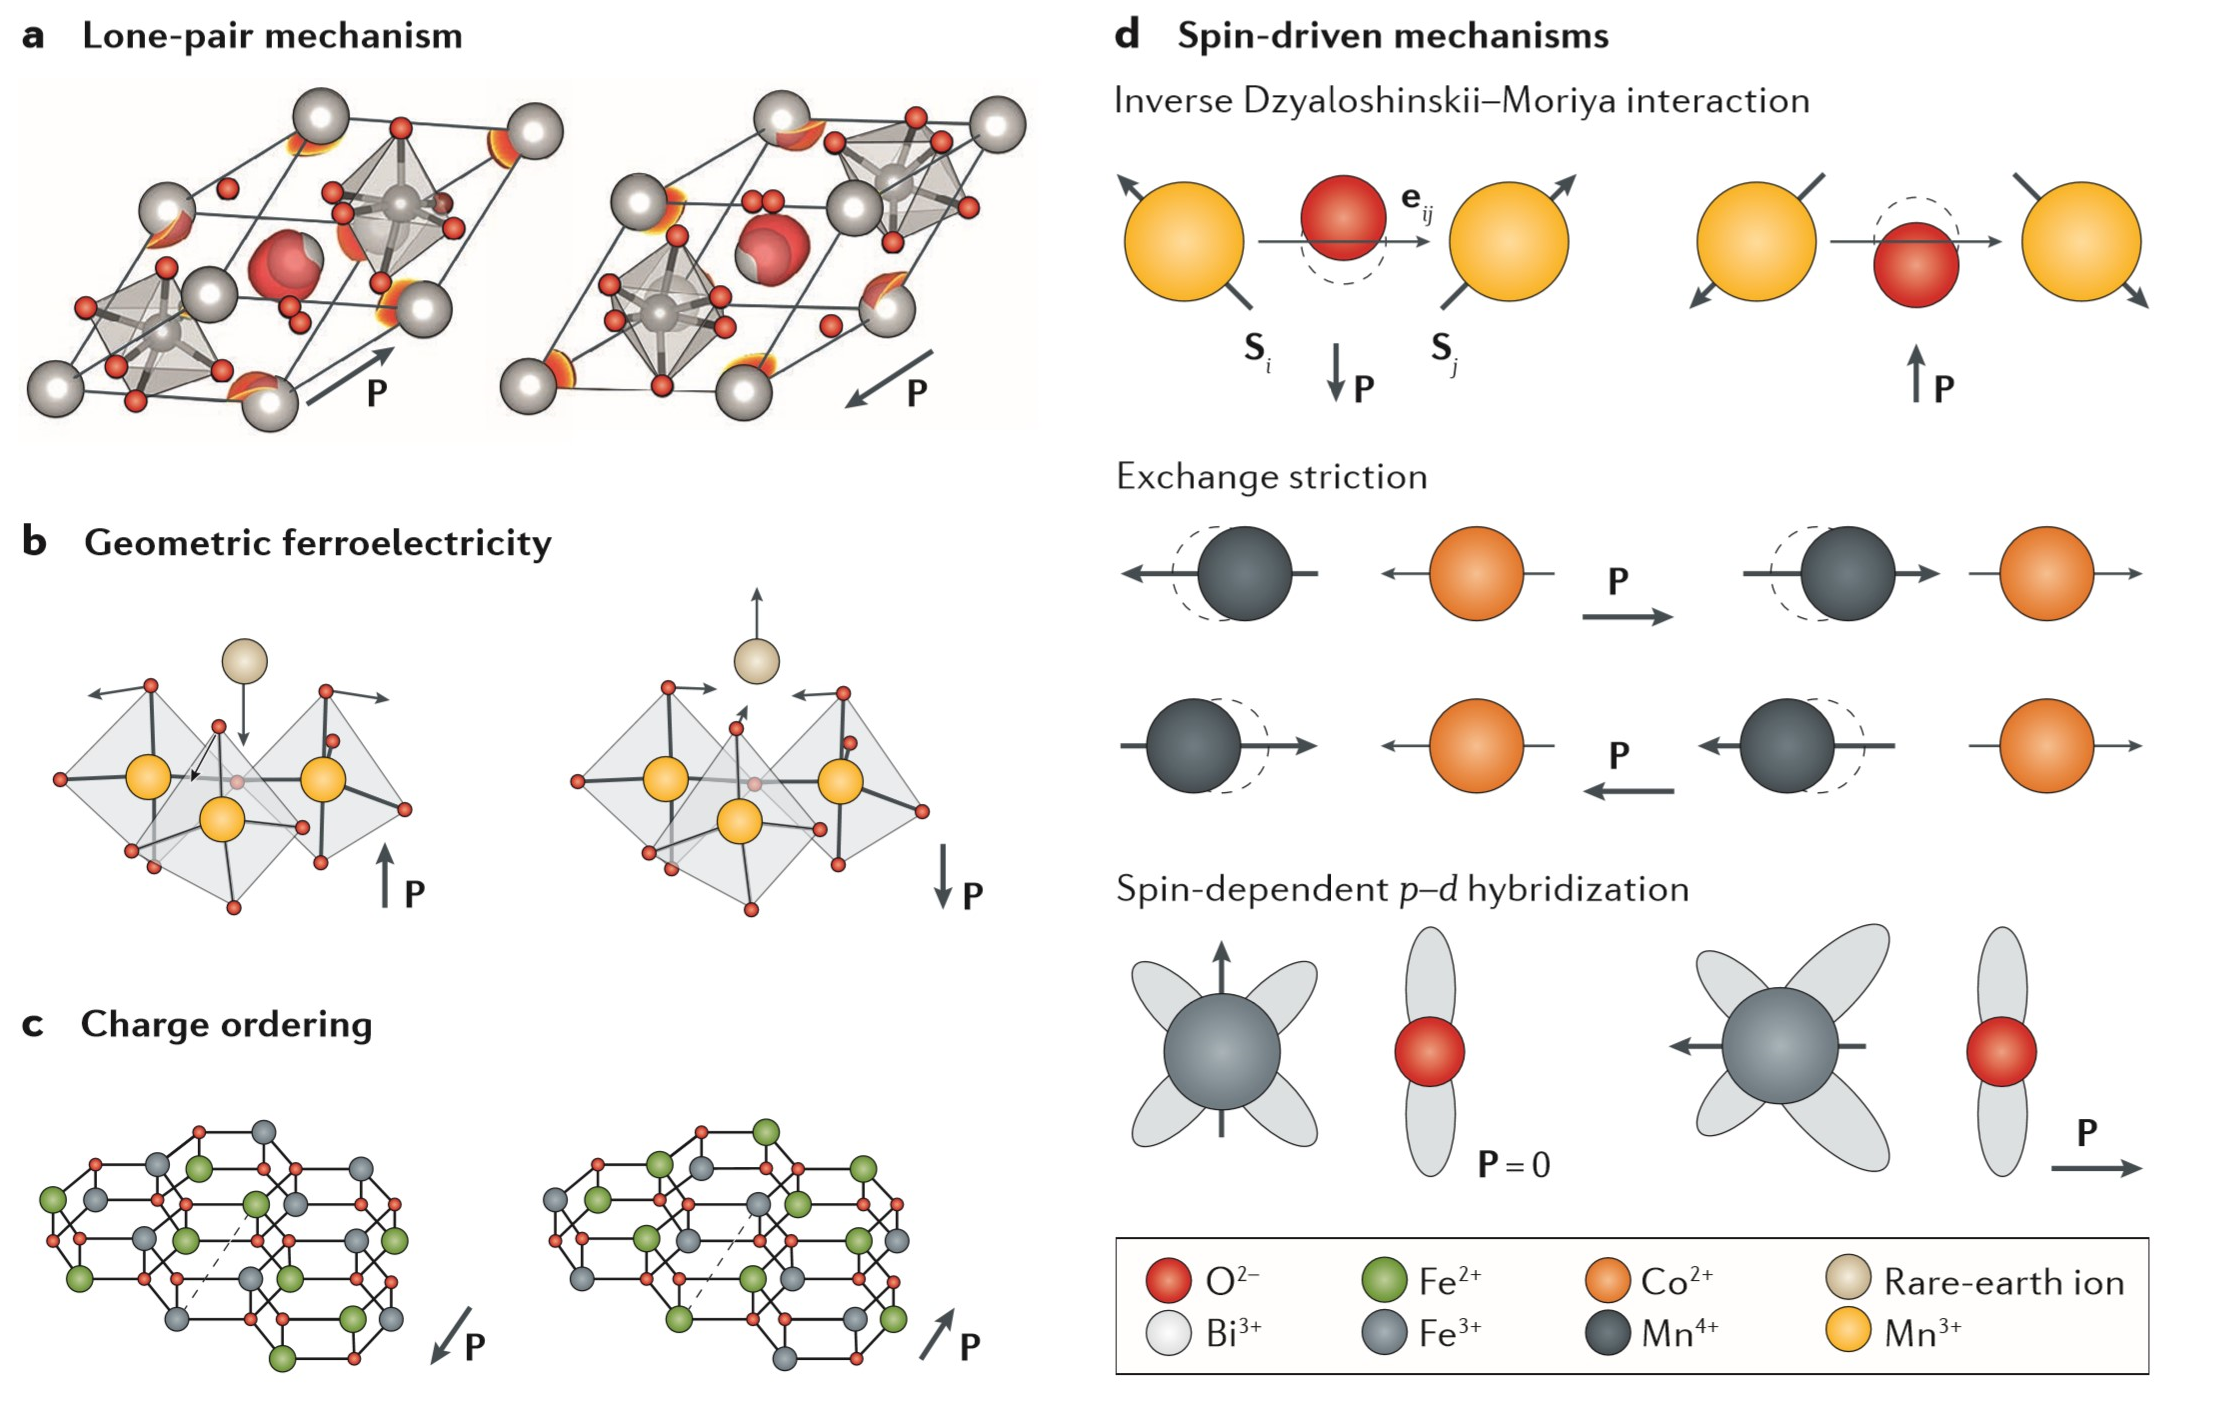
\includegraphics[width=0.8\textwidth]{./pic/006.png}
\caption{多铁材料铁电性的来源机制}
\small
(a)孤对电子机制。典型存在于$BiFeO_{3}$,$Bi^{3+}$离子中的两个电子偏离Bi趋向与氧铁八面体,使晶体内部正负电荷中心偏离,产生了电极化强度。(b)几何机制。典型是$RMnO_{3}$,稀土元素氧离子收到晶格之中氧八面体的几何限制,会在某些方向上面产生电极化。(c)$LuFe_{2}O_{3}$之中的电荷排序。在层状结构之中不同层内$Fe^{3+}$和$Fe^{3+}$的比例不同,这会形成一个电极化。(d)其他的有自旋引起的电极化。主要有Dzyaloshinskii–Moriya作用、交换作用、自旋依赖的p-d轨道杂化等复杂的量子力学相互作用。

\label{dog006}
\end{figure}

\subsection{位形空间中的磁结构}

在实验方面,通过中子衍射可以测量出磁矩在晶格之中的分布,氧化物绝缘体的磁性现象很容易从晶格结构与自旋分布方面解释。例如MnO,其晶体结构与NaCl类似,阴阳离子交替排列。带有自旋磁矩$Mn^{2+}$交替反平行排列,在宏观上没有净磁矩,是典型的反铁磁性。铁氧体是典型的亚铁磁性物质,在$Fe_{3}O_{4}$内部,氧离子按照类似面心立方最密堆积进行排列,金属阳离子只能占据四面体空隙与八面体空隙。在铁氧体内部,按照1:2比例存在着二价铁离子与三价铁离子。通过实验证明,三价铁离子按照1:1的比例填充在八面体与四面体空隙之中,二价铁离子全部填充在八面体空隙之中。八面体空隙之中的自旋与四面体空隙中的阳离子方向反平行。三价铁离子对系统磁矩的贡献相抵消,宏观磁矩实际上是二价铁离子提供的。

\subsection{波矢空间中的磁结构}

在实空间中磁有序可以看做磁矩在周期性格点上的规律排布。磁结构的来源与自旋电子密切相关,在倒格空间之中也可以显示磁现象的能带结构。基于自旋密度泛函的计算结果,可以提供不同自旋取向的磁能带态密度随能量分布曲线。非磁性固体的磁能带是完全对称的,而铁磁性固体有着明显的不对称。不对称导致了不同自旋取向的电子数目不同$N_{\uparrow }\neq N_{\downarrow }$,从而产生自旋极化,可以用来解释金属具有铁磁性的物理起源。


\subsection{铁电性的来源}

铁电性的根源是电极化,通常认为,铁电性来自微观结构之中的电偶极矩,电偶极矩的本质是空间之中的正负电荷中心的不重合。微观结构上空间中的正负电荷有序排列,在宏观就观察到铁电性。从对称性上来看,铁电性的出现是空间反演对称性的破缺。一般来说铁磁性与自发极化需要空的d轨道与孤对电子。

若要获得同时具备铁电性与铁磁性的则需要同时具备以上两种的形式,既要有磁矩又要有电矩,既要有时间反演对称性的破缺又要有空间反演对称性的破缺。

\subsection{多铁材料中的电磁耦合}

单独的铁磁性与铁电性在普通材料之中比较常见,对多铁材料,研究其铁磁性与铁电性的耦合机制有着重要的作用。作为电子自身固有运动的两个属性,电荷与自旋从根本上衍生出电偶极矩与磁矩与铁电性和铁磁性密切相关。研究多铁材料之中铁磁性与铁电性,电荷空间分布与自旋的联系对解开多铁材料的秘密与设计制备新型高性能多铁材料有着重大的理论价值与实践意义。通常认为,多铁材料之中的电磁耦合有三个来源:自旋轨道耦合、自旋晶格耦合与自旋电荷耦合。\cite{nan2019multiferroics}

\paragraph{自旋轨道耦合}
自旋轨道耦合是一种典型的相对论量子力学的结论与效应。运动的电荷产生磁矩,铁磁性的产生与时间反演对称密切相关,电偶极矩的产生与正负电子在空间的分布有关,铁电性的产生与空间电子分布对称性有关。目前看来,能同时联系时间与空间的只有相对论理论,所以解释多铁材料之中电磁耦合的原理应该有来自相对论量子力学的部分。从半经典的角度来看,电子自旋产生磁矩,电子绕核的轨道运动会导致电子在空间中机率密度分布不均衡,特定的轨道运动形式会导致空间对称性的破坏。在一些特殊材料中(例如$TbMnO_{4}$),特殊的磁结构会导致空间反演对称性破话,而自旋轨道耦合会将这种对称性破缺转化为空间中的电偶极矩。相反的如果空间对称性被破坏,自旋轨道耦合也会对磁矩有影响。

\paragraph{自旋晶格耦合}
磁性离子之间的磁相互作用,无论是常规的对称交换作用还是反对称的DM作用,都是取决于电子交换路径的细节。从微观分子角度上看,化学键成键的键长与夹角的改变会对波函数的重叠有影响,进而会影响交换作用。\cite{moriya1960anisotropic}
宏观上的磁致伸缩效应是指在材料在磁场下或者磁化后,宏观上的尺寸会发生变化。压电铁电材料之中的自发极化也会受到晶格畸变的影响,铁磁与铁电性质可以通过晶格结构的改变间接耦合。

\paragraph{自旋电荷耦合}
自旋电荷耦合是由电子密度分布决定的。在磁性系统中,载流子(电子、空穴)可以被自旋极化,因此局域的磁矩可以被电荷密度分布调控,外电场、磁场都可以成为驱动载流子运动的动力。

通常来说,多铁材料内部铁电性与铁磁性耦合很少是由单一原因造成的,通常情况下是由一种原因占主导地位,其余方面处于次要地位。

\subsection{多铁材料的分类}

多铁材料要求同时具有铁电与铁磁两种性质,可以通过两种性质的来源是否相同将多铁材料费为两类,第一类是铁电铁磁两种性质的来源不同,即两种各自独立发挥作用。例如最著名的多铁材料$BiFeO_{3}$\cite{姚携菲2014磁电多铁性材料的宠儿},其中$Bi^{3+}$提供孤对电子,在晶体结构内部产生一个电偶极矩,三价铁离子提供磁矩。两种因素相互配合,使其在宏观上同时表现出铁电性与铁磁性。第二类多铁材料是指材料的铁磁性与铁电性是同源的。\cite{段纯刚2009磁电效应研究进展} 多铁材料可以根据多铁性的具体来源可以进行进一步的细分。



\paragraph{复合多铁材料}
这种多铁材料的产生原理并不复杂,把一种只有铁电性的材料,例如$BaTiO_{3}$与一种只有铁磁性的材料,如$CoFe_{2}O_{4}$混合起来,一层一层叠加在一起,层层生长形成超晶格,在室温下实现了磁场与电场的耦合,并可以通过控制磁场的方式影响电极化。其优点是耦合强度高,在室温下稳定存在。但这样层叠复合材料就不是单相材料了,另外,利用电场控制磁场的效应仍待进一步研究。\cite{vaz2010magnetoelectric}

\paragraph{孤对电子机制}
这种多铁材料是单相的,一般包含两种及以上的阳离子,一种提供孤对电子与铁电性质,另一种提供磁铁性。上文提到的$BiFeO_{3}$就属于这一种。$BiFeO_{3}$是一种在室温下,具有强电磁耦合的,稳定的电极化的单相多铁材料。

铁酸铋是多铁材料之中比较重要的一个,经过数十年的发展,进行过大量的研究。铁酸铋的铁电极化与磁有序的耦合在室温以上的温度下依然存在。$BiFeO_{3}$蕴含着大量的新物理与潜在应用,其内部存在的T型结构与R型结构仍待研究,其独特的光电效应光催化、光摩擦、光变色、气体敏感、表面现象是研究的热点。\cite{姚携菲2014磁电多铁性材料的宠儿} 

\paragraph{几何驱动的铁电性}
这种材料的铁电性的来源是几何性质的因素。某些几何学上的限制会导致结构不稳定,从而使某些离子位移,进而产生电偶极矩。例如一个小的阳离子可以允许周围的配位多面体旋转,这些配位多面体本身带有极性。这类材料的代表是$BaNiF_{4}$,这些新开发的材料在铁电性上都不如传统铁电材料,主要的阶数参数是转动阶数,而不是铁电极性畸变。改良这类材料的关键是对铁电性的具体机制进行研究。\cite{fox1977ferroelectrically} 

\begin{figure}[h]
    \centering
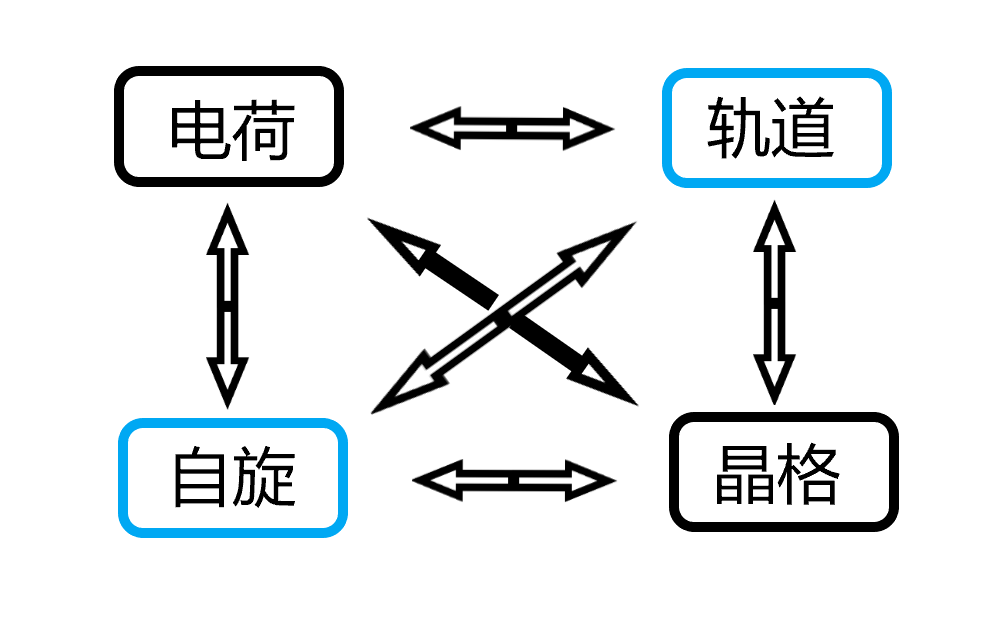
\includegraphics[width=0.8\textwidth]{./pic/008.png}
\caption{多铁材料中的电磁耦合}

\label{dog008}
\end{figure}

\paragraph{电荷排序} 
价电子在主要离子周围的分布可能是不均匀不对称的,这在晶体结构上可能会产生一个电偶极矩。主要的例子是$LuFe_{2}O_{4}$,其内部的三价铁离子与二价铁离子在不同层间的比例不同,不仅破坏了空间反演,这导致了电荷在空间的有序排列以及层间的电偶极矩。\cite{qin2015an}

\paragraph{自旋驱动的铁电性}
这类多铁材料是一种铁电铁磁同源的多铁材料,电子自旋不仅引起了铁磁性,而且还产生了电极化。目前认为自旋引起的极化可能有三种来源:DM(Dzyaloshinskii–Moriya)相互作用\cite{dzyaloshinsky1958thermodynamic}、类海森堡的交换作用、依赖自旋的轨道杂化。铁电铁磁同源的铁电材料的电磁耦合强度是最高的。